\documentclass[11pt]{ctexart}
\usepackage[top=2cm, bottom=2cm, left=2cm, right=2cm]{geometry}
\usepackage{algorithm}
\usepackage{algorithmicx}
\usepackage{algpseudocode}
\usepackage{amsmath}
\usepackage{graphicx}
\usepackage{listings}
\usepackage{xcolor}
\usepackage{float}
\usepackage{amsmath}
\usepackage{bm}
\usepackage{autobreak}
\usepackage{amssymb}
\usepackage{listings} %插入代码
\usepackage{xcolor} %代码高亮

\floatname{algorithm}{算法}
\renewcommand{\algorithmicrequire}{\textbf{输入:}}
\renewcommand{\algorithmicensure}{\textbf{输出:}}

\lstset{numbers=left, %设置行号位置
        numberstyle=\tiny, %设置行号大小
        keywordstyle=\color{blue}, %设置关键字颜色
        commentstyle=\color[cmyk]{1,0,1,0}, %设置注释颜色
        frame=single, %设置边框格式
        escapeinside=``, %逃逸字符(1左面的键),用于显示中文
        breaklines, %自动折行
        extendedchars=false, %解决代码跨页时,章节标题,页眉等汉字不显示的问题
        xleftmargin=2em,xrightmargin=2em, aboveskip=1em, %设置边距
        tabsize=4, %设置tab空格数
        showspaces=false %不显示空格
}

%
\makeatletter
\def\lst@lettertrue{\let\lst@ifletter\iffalse}
\makeatother
%

\title{\huge\bf
算法设计大作业(二)}
\author{毛圆鑫 - 201721012271}
\date{\today}

\begin{document}
\maketitle
\section*{说明}
这是算法设计课的第二个大作业,主题是\textbf{动态规划算法的分析},我完成的题目是\textbf{第二道}:求解最短公共超串。

在\textbf{题目描述}中有完整的题目介绍,之后便是我的分析报告,整篇文档是基于 \LaTeX 语言设计的,源码见附件或github.com/punk-boy/algorithm/dynamicprogram.tex和dynamicprogram.cpp


\section{题目描述}
令$A[1\dots n]$和$B[1\dots n]$是两个任意的字符串。A、B的超串是指存在某个字符串C,使得A和B都是它的子串。要求:给定字符串A和B,请编写一个算法,计算A和B的最短公共超串,并输出该串的长度。

\section{问题理解}
这里我们讨论一下,题目的中的最短公共超串的定义,百度和谷歌都没有给出这个定义,为了下面讨论方便,我们认为$C$串中存在和$A$串相同的序列时,$C$串中存在和$B$串中相同的序列时,我们就叫$C$串是的公共超串。这是跟老师讨论过的。如果你对这个定义有所疑惑,可以在阅读完文章中的大部分内容后,阅读“附录”内容,那里我给出了一些解释。

这个问题按照我们上面的规定,其实和最长公共子序列十分的类似,如此,我们便可以参考着最长公共子序列的动态规划的证明和解法来求解该问题。

\section{形式化描述}
其实这道题目以及很抽象了,不需要再加一个形式化的描述了,但是为了行文的完整性,这里还是给出一个形式化描述:

\textbf{子序列的定义:}

给定$A$串为$\{a_1, a_2, \dots, a_n\}$,$Z$串为$\{z_1, z_2, \dots, z_m\}$,存在一个严格递增的下标序列$\{i_1,i_2,\dots,i_k\}$,使得对于任何的$j=1,2,\dots,k$,有$z_j=x_{x_j}$,则称$Z$是$X$的子序列。

按照我们的规定,\textbf{公共超串的定义:}

给定两个序列$X$和$Y$,若存在另一个序列$Z$同时是$X$和$Y$的子序列,我们就称$Z$是$X$和$Y$的最短公共超串。

\section{朴素解法}
将$A$串为$\{a_1, a_2, \dots, a_m\}$和$B$串$\{b_1, b_2, \dots, b_n\}$拼接在一起组成一个临时的字符串$S$为 \\ $\{s_1, s_2,\dots, s_{m+n}\}$,我们找出$S$字符串的所有子序列,并在过程中检查$A$和$B$是不是$Q$的子序列,在此过程中记录最短的$Q$。最终,我们找到的最短的$Q$就是$A$和$B$的最短公共超串。

这样做的话,时间复杂度是很大的:
\begin{enumerate}
    \item 拼接$A$串,$B$串成为$S$串,为$O(1)$;
    \item 求出$S$串的所有的子序列$Q$,每位都有取和不取两种状态,所以时间复杂度为$O(2^{m+n})$;
    \item 在取到子序列的过程中,我们都要判断$A$和$B$是不是$Q$的子序列,这个时间复杂度是$O(m+n)$
    \item \textbf{结论:根据大O公式的乘法、加法性质,时间复杂度为:$O((m+n)2^{m+n})$}
\end{enumerate}

\section{动态规划可行性证明}
设$A$串$\{a_1, a_2, \dots, a_m\}$,$B$串$\{b_1, b_2, \dots, b_n\}$,有最短公共超串$C$为$\{c_1, c_1, \dots, c_k\}$

\subsection{重叠子问题性质}

\begin{figure}[H]
	\centering
	\includegraphics[]{dynamicprogram.eps}
	\caption{最短公共超串问题的重叠子问题}
	\label{}
\end{figure}

大家通过递归树,也就可以看出重叠子问题了吧。

\subsection{最优子结构性质}

\subsubsection*{一、\\如果$a_m=b_n$,那么$c_k=a_m=b_n$,且$c_{k-1}$是$a_{m-1}$和$b_{n-1}$的最短公共超串}

\noindent \textbf{证明:}\bm{$c_{k} = a_{m} = b_{n}}$
假设$c_k \neq a_m$,则说明$k'<k$。使得$c_{k'} = a_m$,

这时,那么$c_{k} = b_n$,因为我们没法保证$c_{k'} = c_{k}$,所以这就使得$a_m \neq b_n$,假设不成立。


%假设$c_k \neq a_m$。

%因为$c_k$是$a_m$和$b_n$的最段公共超串,存在严格递增的下标序列${i_1,i_2,\dots ,i_k}$,使得对于任意$j=1,2,…,k,$有$c_j=a_{i_j}$;

%由于$c_k \neq a_m$,说明$i_k<m$.这时,将$i_{k+1}=m$增加到下标序列中,就得到一个新的下标序列${i_1,i_2,…,i_k,i_{k+1}}$。显然,该序列满足对于任意$j=1,2,\dots,k,k+1$,有$c_j=a_{i_j}$.
%这说明$a_m$和$b_n$有一个长度为$(k+1)$的公共子序列$c_{k+1}$,这与$c_k$是$a_m$和$b_n$的最段公共超串矛盾,假设不成立。

\noindent \textbf{证明:$c_{k-1}$是$a_{m-1}$和$b_{n-1}$的最短公共超串}

假设$c_{k-1}$不是$a_{m-1}$和$b_{n-1}$的最短公共超串

则说明$a_{m-1}$和$b_{n-1}$存在一个长度小于$(k-1)$的公共超串,不妨设它们有一个长度为$k’$的公共子序列$D_{k’}$

将符号$c_k=a_m=b_n$增加到$D_{k’}$的末尾,就得到了一个长度为$(k’+1)$的序列。显然,该序列是$a_m$和$b_n$的最短公共超串,且长度为$k’+1<(k-1)+1=k$。

这与$c_k$是$a_m$和$b_n$的最长公共子序列的前提矛盾,所以假设不成立。

\subsubsection*{二、\\若$a_m \neq b_n$,且$c_k\neq a_m$,则$c_k$是$a_{m-1}$和$b_n$的最短公共超串\\
	若$a_m \neq b_n$,且$c_k\neq b_n$,则$c_k$是$a_m$和$b_{n-1}$的最短公共超串}

\noindent\textbf{证明(我们只证明第一个,第二条性质同理可证):}

假设$c_k$不是$a_{m-1}$和$b_n$的最短公共超串。

说明$a_{m-1}$和$b_n$存在一个长度小于$k$的最短公共超串,不妨设该序列的长度为$k’$。

$c_{k’}$是$a_{m-1}$和$b_n$的公共超串,显然它也是$a_m$和$b_n$的公共超串,并且$k’<k$。

这与$c_k$是$a_m$和$b_n$的最短公共超串的前提矛盾.假设不成立.


\section{动态规划解法思路}
设dp[i][j]表示序列$A$和$B$串的最短公共超串$C$的长度,则有:
$$
c[i][j]=\left\{ \begin{array}{ll}
\max\{i,j\},&i=0 \quad or \quad j=0\\
c[i-1][j-1]+1,&i,j>0 \quad and \quad x_i=y_j\\
min\{c[i-1][j], c[i][j-1]\}+1 ,&i,j>0 \quad and \quad x_i\neq y_j\\
\end{array}\right.
$$

\section{伪代码}
\begin{algorithm}[H]
\caption{求解最短公共超串}
\begin{algorithmic}[1] %每行显示行号
\Require 字符数组$X[]$及其长度$m$,字符数组$Y[]$及其长度$n$,动态规划数组$dp[][]$,动态规划过程数组$b[][]$
\Ensure 最短公共超串的长度
\Function {ShortestCommonString}{$X[], Y[], m, n$}
\State $dp[i][j] \gets 0$
\For{$i=0 \to m$}
    \State $dp[i][0]=0,b[i][0]\gets '\uparrow'$
\EndFor
\For{$j=0 \to n$}
    \State $dp[0][j]=0,b[0][j]\gets '\leftarrow'$
\EndFor
\For{$i=0 \to m$}
    \For{$j=0 \to n$}
        \If{$X[i]=Y[i]$}
            \State $dp[i][j] \gets dp[i-1][j-1]+1, b[i][j] \gets '\nwarrow'$
        \ElsIf{$dp[i-1][j] \leqslant dp[i][j-1]$}
            \State $dp[i][j] \gets dp[i-1][j]+1, b[i][j] \gets '\uparrow'$
        \Else
            \State $dp[i][j] \gets dp[i][j-1]+1, b[i][j] \gets '\leftarrow'$
        \EndIf
    \EndFor
\EndFor
\Return{$c[m][n]$}
\EndFunction
\end{algorithmic}
\end{algorithm}

\section{代码实现}
为了简化篇幅,这里只给出对应方法的实现,案例、对结果的回溯查看以及更加详细的源代码信息,请查看附件中的.cpp文件或是通过GitHub找到对应的.cpp文件。
\begin{lstlisting}[language=C++]
int shortest_common_string(char * x, char * y, int m, int n)
{
	dp[0][0] = 0;
	b[0][0] = 0;
	for(int i=1;i<=m;i++)
	{
		dp[i][0] = i;
		b[i][0] = 'U';
	}
	for(int j=1;j<=n;j++)
	{
		dp[0][j] = j;
		b[0][j] = 'L';
	}
	for(int i=1;i<=m;i++)
	{
		for(int j=1;j<=n;j++)
		{
			if(x[i-1] == y[j-1])
			{
				dp[i][j] = dp[i-1][j-1]+1;
				b[i][j] = 'O';
			}
			else if(dp[i-1][j] <= dp[i][j-1])
			{
				dp[i][j] = dp[i-1][j] + 1;
				b[i][j] = 'U';
			}
			else
			{
				dp[i][j] = dp[i][j-1] + 1;
				b[i][j] = 'L';
			}
		}
	}
	return dp[m][n];
}
\end{lstlisting}

\section{实验结果}
\begin{figure}[H]
\centering
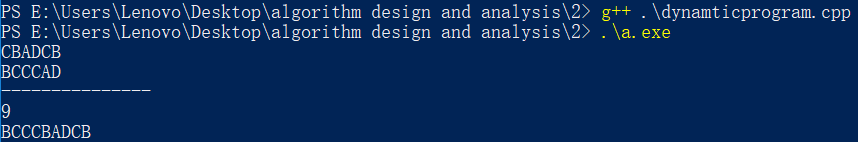
\includegraphics[scale=0.9]{dynamticprogram.png}
\caption{最短公共超串的实验结果}
\end{figure}
\section{复杂度分析}
动态规划的题目嘛,好像也没有说明时间复杂度可以分析,两重循环用于计算$dp$数组,故$T(n) = O(n^{2})$,空间复杂度也很easy,$S(n) = O(n^{2})$。

\section{后续优化和感想}
可以通过改进动态规划中数组的使用,使得空间复杂度由$O(n^{2})$降到$O(n)$。

这是我第二次做有关于动态规划的题目的分析(很巧,我上次的题目是一道纯正的动态规划题),已经理解了很多,想想大一,二时费劲脑汁的推导各种动态规划算法的递推解是,我只想说,要不学院考虑考虑把这门课提早一个学期开,最后,感谢一下老师,讲的真的很好,算法是个很难的一块,动态规划更是有点生涩,老师真的讲的清楚明白。

\section{附录}
原题目:令$A[1\dots n]$和$B[1\dots n]$是两个任意的字符串。A、B的超串是指存在某个字符串C,使得A和B都是它的子串。

如果按照我们平常理解子串的想法,则这道题目是不适合用动态规划解的,比如ABCD和EDCBAZ这两个串,动态规划的过程中一直都找不到一个合适的解,原因在于第一个元素就不相同,同理,从后往前找,也是这样。所以这个问题的最好解法是通过贪心,通过比较A串的头和B串的尾,或A串的尾和B串的头,如果这两个情况的结果都是0,则A和B的最短公共超串一定是两个字符串的拼接。

而如果使用了序列的是想,则这个问题就有的讨论了,因为序列并不需要连续。

最后,再说说为什么选这道题目呢:三个动态规划例子中,就属最优子结构性质学得稀里糊涂的,借这个机会回顾一下最短子序列的最优子结构性质。

\end{document}



